% !TEX root = ../main.tex

\begin{frame}{Microphones}
	\begin{itemize}
		\item We prefer headset microphones over handheld for speakers
		\item Distance to mouth will be constant -> more consistent audio level
		\item Handheld microphones for heralds and Q\&A
		\item Our transmitters also have a mute button (yellow light = muted)
		\item Please check battery level from time to time
	\end{itemize}
\end{frame}

\begin{frame}{Headset Placement}
	\begin{columns}[T,onlytextwidth]
		\column{0.6\textwidth}
		\begin{figure} 
			\centering
			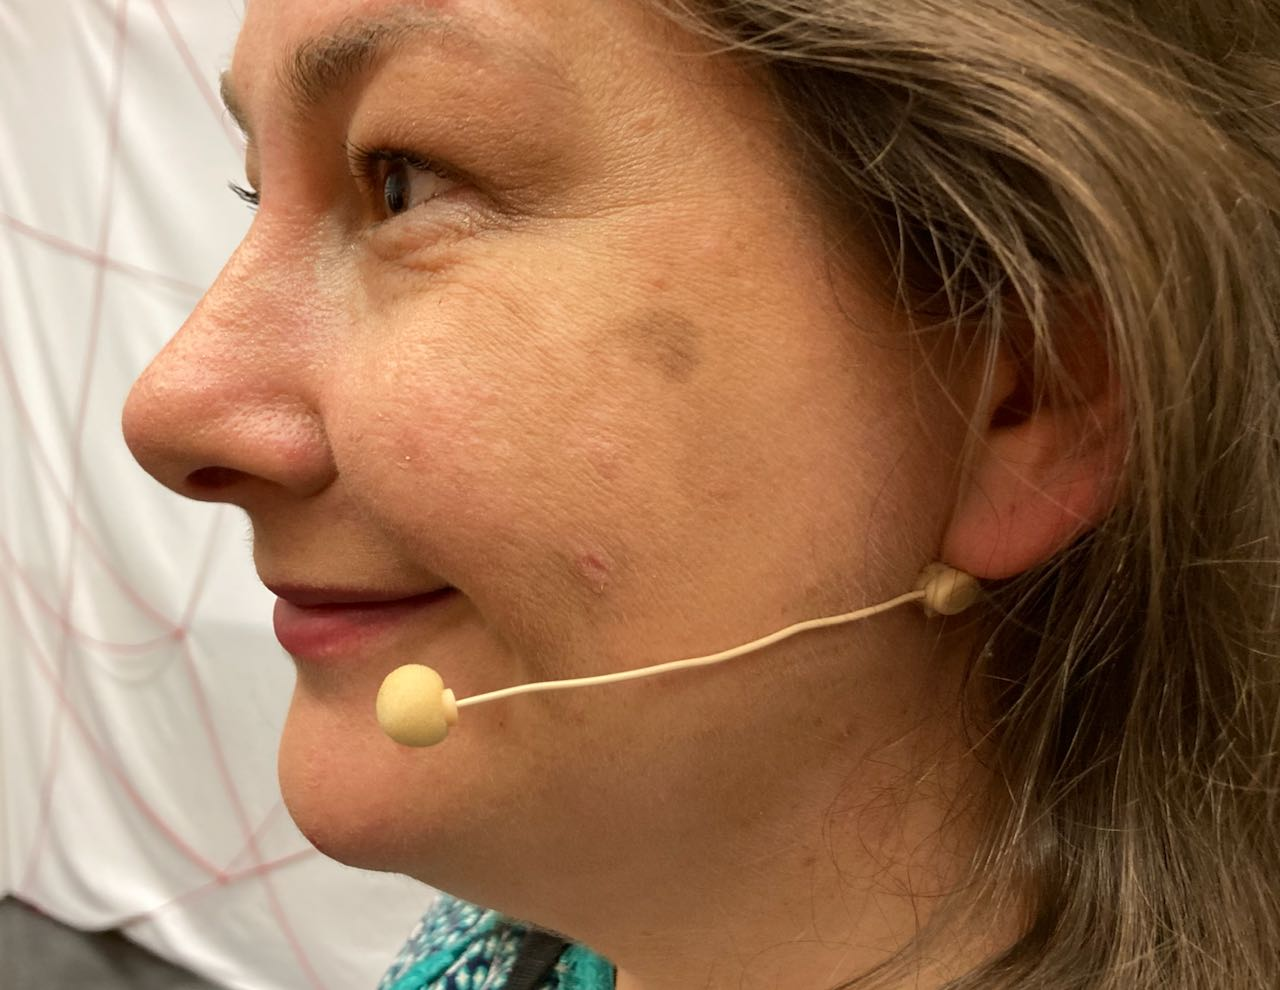
\includegraphics[width=0.9\textwidth]{images/headset-side.jpeg}
			\caption{Good headset microphone placement}
		\end{figure}
		\column{0.4\textwidth}
		\begin{itemize}
			\item Microphone shall be at the corner of the mouth
			\item Boom can slide back and forth
			\item If too far in front, there will be too much wind noise
			\item Distance to face: About 2 cm
			\item Bend boom carefully
		\end{itemize}
	\end{columns}
\end{frame}
